\documentclass{isabec} % Specifies the document class

%% The preamble begins here.
\usepackage[super,comma,round]{natbib}
\usepackage[figuresleft]{rotating}
\usepackage{txfonts}

% Metadata Information
\jyear{XXXX}%% conference year
\jnumber{MANUSCRIPT-NUMBER} %% manuscript number

%% Document starts
\begin{document}
\markboth{Author et al.}{MANUSCRIPT-NUMBER}

% Title
\title{Title title title title title title title title title title}
\subtitle{Subtitle subtitle subtitle subtitle subtitle subtitle subtitle}

%% Authors, affiliations address.
% Corresponding author
\author{A. Author One\email{abcd.xyz@mnop.edu}\\ B. Name Author Two\thanks{{\bf Author's notes}}}
\affil{Affiliation One\\ Department Name\\ City Name\\ Country Name}

% Co-authors
\author{A. Author One, B. Author Two and C. Author Three}
\affil{Affiliation Two\\ Department Name\\ City Name\\ Country Name}
\author{A. Author One and C. Author Two}
\affil{Affiliation Three\\ Department Name\\ City Name\\ Country Name}

% Produces the title
\maketitle                   

% Abstract
\begin{abstract}
Dummy Text of abstract. Dummy Text of abstract. Dummy Text of abstract. Dummy Text of abstract. Dummy Text of abstract. Dummy Text of abstract. Dummy Text of abstract. Dummy Text of abstract. Dummy Text of abstract. Dummy Text of abstract. Dummy Text of abstract. Dummy Text of abstract. Dummy Text of abstract. Dummy Text of abstract. Dummy Text of abstract. Dummy Text of abstract. Dummy Text of abstract. Dummy Text of abstract. Dummy Text of abstract. Dummy Text of abstract. Dummy Text of abstract. Dummy Text of abstract. Dummy Text of abstract. Dummy Text of abstract. Dummy Text of abstract. Dummy Text of abstract. Dummy Text of abstract. Dummy Text of abstract. Dummy Text of abstract. Dummy Text of abstract. Dummy Text of abstract. Dummy Text of abstract. Dummy Text of abstract.
\end{abstract}

% Nomenclature
\section*{NOMENCLATURE} % head one
\begin{deflist}% Nomenclature text start here%
\listterm{a}{dummy text}
\listterm{a, b}{dummy text dummy text}
\listterm{\emph{APU}}{dummy text dummy text}
\listterm{ci}{dummy text dummy text}
\listterm{CT}{dummy text}
\listterm{\emph{CAS}}{dummy text dummy text}
\listterm{E}{dummy text}
\listterm{D}{dummy text}
\listterm{f}{dummy text}
\listterm{Fg}{dummy text}
\listterm{F}{dummy text}
\listterm{\emph{FCOM}}{dummy text}
\end{deflist}

\subsection*{Greek Symbol}% head two of nomenclatrue
\begin{deflist}
\listterm{$\alpha$}{dummy text}
\listterm{$\beta$}{dummy text dummy text}
\listterm{$\gamma$}{dummy text dummy text}
\listterm{$\delta$}{dummy text dummy text}
\listterm{$\xi$}{dummy text dummy text}
\listterm{$\phi$}{dummy text dummy text dummy text dummy text dummy text dummy text dummy text dummy text dummy text dummy text dummy text dummy text dummy text dummy text}
\listterm{$\psi$}{dummy text dummy text}
\end{deflist}


% Heading 1
\section{INTRODUCTION}
Please begin the main text of your article here.

%Heading 1
\section{FIRST-LEVEL HEADING}% Head A
This is an example of dummy text.

\subsection{Second-Level Heading}% Head B
This is an example of dummy text. This is an example of dummy text.

% Heading 3
\subsubsection{Third-Level Heading}
This is dummy text. This is dummy text. This is dummy text. This is dummy text. 

% Heading 4
\paragraph{Fourth-Level Heading} %Fourth-level headings
This is dummy text. This is dummy text. This is dummy text. This is dummy text. 

% Example of a single-line equation
\subsection{Equations}
Example of a single-line equation \ref{eqn1}
\begin{equation}
a = b \ {\rm ((Single\ Equation\ Numbered))}\label{eqn1}
\end{equation}
% Example of a single-line unnumbered equation
\[
a = b \ {\rm ((Single\ Equation\ Unnumbered))}
\]
%Example of multiple-line numbered equation
Equations can also be multiple lines as shown in Equation \ref{eqn2} and \ref{eqn3}.
\begin{eqnarray}
c = 0 \ {\rm ((Multiple\  Lines, \ Numbered))}\label{eqn2}\\
ac = 0 \ {\rm ((Multiple \ Lines, \ Numbered))}\label{eqn3}
\end{eqnarray}

% Example of multiple-line unnumbered equation
Equations can also be multiple lines as shown below:
\begin{eqnarray}
c = 0 \ {\rm ((Multiple\  Lines, \ Unnumbered))}\nonumber\\
ac = 0 \ {\rm ((Multiple \ Lines, \ Unnumbered))}\nonumber
\end{eqnarray}


% Example of lists
\subsection{Examples of Lists}
Here is an example of a numbered list.
\begin{enumerate}
      \item First numbered list item...
      \item Second numbered list item...
      \item Third numbered list item...
\end{enumerate}
%
\textbf{Here is an example of a bulleted list.}
\begin{itemize}
  \item This is an example of bulleted list.
  \item This is an example of bulleted list.
  \item This is an example of bulleted list.
\end{itemize}
%
\textbf{Here is an example of a unnumbered list.}
\begin{unnumlist}
  \item First unnumbered item...
  \item Second unnumbered item...
  \item Third unnumbered item...
\end{unnumlist}
%
\textbf{Numbered list with parenthesis}
\begin{arabiclist}% (1), (2), (3), .....
  \item First numbered list item (1)...
  \item Second numbered list item (2)...
  \item Third numbered list item (3)...
\end{arabiclist}
%
\textbf{Alpha list with parenthesis}
\begin{alphalist}% (a), (b), (c) ....
  \item First numbered list item...
  \item Second numbered list item...
  \item Third numbered list item...
\end{alphalist}
%
\textbf{Small roman list.}
\begin{romanlist}% (i), (ii), (iii), .....
  \item First numbered list item...
  \item Second numbered list item...
  \item Third numbered list item...
\end{romanlist}
%
\textbf{Capital Roman list.}
\begin{Romanlist}% I., II., III., ......
  \item First numbered list item ...
  \item Second numbered list item ...
  \item Third numbered list item ...
\end{Romanlist}
%

\subsection{Here is an example of extract}
This is an example of extract

\begin{extract}
This is an example text of quote or extract. This is an example text of quote or extract. 
This is an example text of quote or extract. This is an example text of quote or extract.
This is an example text of quote or extract. This is an example text of quote or extract. 
This is an example text of quote or extract. This is an example text of quote or extract.
This is an example text of quote or extract. This is an example text of quote or extract. 
This is an example text of quote or extract. This is an example text of quote or extract.
\end{extract}

\subsection{Footnote}
This is an example of footnote\footnote{This is an example of a footnote.}.

\subsection{Example of Enunciations}  
Example of theorem \ref{thm1}, lemma \ref{lem1} and remark \ref{rem1}
%% Theorem 1
\begin{theorem}\label{thm1}
Example of theorem Example of theorem Example of theorem Example of theorem
Example of theorem Example of theorem Example of theorem Example of theorem
\[ a+b= c \]
\end{theorem}
%% Lemma 1
\begin{lemma}\label{lem1}
Example of lemma. Example of lemma. Example of lemma. Example of lemma. Example of lemma. Example of lemma
\end{lemma}
%% Theorem 2
\begin{theorem}[Math Detail one]\label{thm2}
Example of theorem with math detail
\end{theorem}
% Remark 1
Example of remark \ref{rem1}
\begin{remark}[Math Detail]\label{rem1}
Example of remark with math detail
\end{remark}

\begin{proposition}
Example of proposition
\end{proposition}

\begin{corollary}
Example of corollary
\end{corollary}

\begin{definition}
Example of definition
\end{definition}

\begin{assumption}
Example of assumption
\end{assumption}

\begin{notation}
Example of notation
\end{notation}

\begin{claim}
Example of claim
\end{claim}

\begin{proof}
Example of proof Example of proof Example of proof Example of proof Example of proof Example of proof Example of proof Example of proof Example of proof 
\end{proof}

% Example of a Figure
\subsection{Figures}
Figures should be cited in the main text in chronological order. This is dummy text with a citation to the first figure which is shown as Fig.~\ref{fig1}. Figure~\ref{fig1} shows that dummy text dummy text.

\begin{figure}[h]
\begin{center}
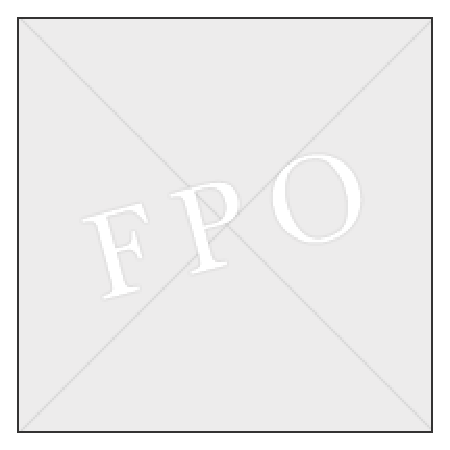
\includegraphics[width=3in,height=1.2in]{fpo}% SampleFigure is name of eps%
\end{center}
\caption{This is an example of a figure caption.}
\label{fig1}
\end{figure}\vspace*{-12pt}

\subsection{Tables}
Tables should also be cited in the main text in chronological order Table \ref{tab1}.

\begin{table}[h]
\tabcolsep7.5pt
\caption{Table caption}
\label{tab1}
\centering
\begin{tabular}{@{}lcccc@{}}
\textbf{Head 1} &\multicolumn{3}{c}{{\bf Span of Column 2,3,\&4}}&\textbf{Head 5}\\
\textbf{{(}units)$^{\rm a}$} &\textbf{Head 2} &\textbf{Head 3} &\textbf{Head 4} &\textbf{{(}units)}\\[6pt]
Column 1 &Column 2 &Column3$^{\rm b}$ &Column4 &Column\\
Column 1 &Column 2 &Column3 &Column4 &Column\\
Column 1 &Column 2 &Column3 &Column4 &Column\\
Column 1 &Column 2 &Column3 &Column4 &Column\\
\end{tabular}
\begin{tabnote}
$^{\rm a}$Table footnote\\ $^{\rm b}$second table footnote.
\end{tabnote}
\end{table}

\pagebreak

\subsection{Small figures to be generated side by side}
\begin{figure}[h]
\centering
\begin{minipage}[b]{.45\textwidth}
\centering
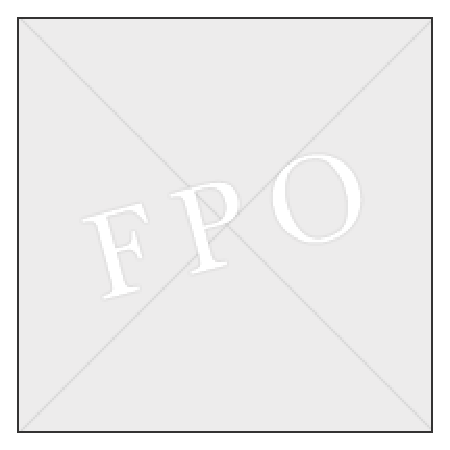
\includegraphics[width=1in,height=1.2in]{fpo}%
\caption{\hsize15pc This is an example of a figure caption}\label{fig2}
\end{minipage}\hfill
%
\begin{minipage}[b]{.45\textwidth}
\centering
 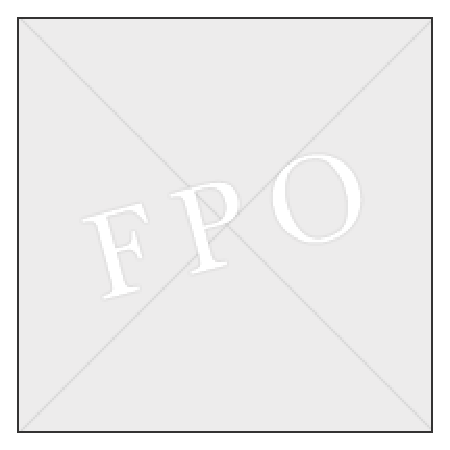
\includegraphics[width=2in,height=1.2in]{fpo}%
 \caption{This is an example of a figure caption. This is an example of a figure caption.}\label{fig3}
\end{minipage}
\end{figure}


\vspace*{-15pt}
\section*{ACKNOWLEDGEMENTS}
This is an example of acknowledgement\cite{author1,author2}. This is an example of acknowledgement\cite{author3}. This is an example of acknowledgement. This is an example of acknowledgement\cite{author4}.

% References
\begin{thebibliography}{0}%{00}%{000}
\bibitem{author1}
\textsc{Author One, B.C.} and \textsc{Author Two, D.} A framework for aircraft conceptual design and environmental performance studies, \textit{BIBB J}, October 2009, \textbf{52}, (10), pp 2100-2109.

\bibitem{author2}
\textsc{Author One, B.C.}, \textsc{Author Two, D.} and \textsc{Author Three, D.} Towards a silent aircraft, \textit{Aeronaut J}, August 2006, \textbf{110}, pp 487-494.

\bibitem{author3}
\textsc{Author Surname, B.} Advanced Aircraft Flight Performance, 2012, Cambridge University Press.

\bibitem{author4}
\textsc{Author, C.} Comprehensive analysis of transport aircraft flight performance, \textit{Prog Aerospace Sci}, April
2007, \textbf{43}, (3), pp 192-236.

\end{thebibliography}

\setcounter{section}{0}
%%%%%%% Appendix
\section*{APPENDIX}
\section{FIRST ORDER HEADING}

\begin{table}[h]
\tabcolsep8pt
\caption{Table caption table caption table caption table caption table caption table\break caption table caption table caption table caption table caption table\break caption table caption table caption table caption}
\label{tab4}
\centering
\begin{tabular}{@{}lccccc@{}}
%% table column head start%
&{\bf Column 2}&\multicolumn{2}{c}{{\bf Span Col 3\&4}} &\multicolumn{2}{c}{{\bf Span Col 5\&6}}\\
{\bf Column 1} &{\bf Column 2} &{\bf Column 3} &{\bf Column 4} &{\bf Column 5} &{\bf Column 6}\\[6pt]
%%Table body start
6--31 $+$ G(d,p) &460 &2.12 &1.04 &8.63 &3.48\\
6-311 $+$ G(d,p) &572 &2.86 &1.29 &11.90 &4.56\\
6-311 $+$ $+$ G(3df,2p) &1,060 &7.54 &3.25 &36.70 &11.45\\
\end{tabular}
\begin{tabnote}
$^{\rm a)}$Table Footnote; $^{\rm b)}$ Second Table Footnote.
\end{tabnote}
\end{table}

% End of document.
\end{document}               
